\chapter{実装}
\label{chap:implementation}

実装がまだ完成してないので,空想です.

\section{実験環境}

本研究で実装を行う環境は,RDMA NICが刺さった監視対象ホストと,本研究における実装を実行するホストの2台で構成する.

監視対象ホストは,Linux 4.15.0-72-genericのubuntuであり,PCIeデバイスとして,FPGAボードが刺さっている.
このFPGAボードは,\ref{chap:related_works}章にて述べたように,dma messageとethernetパケットを相互変換する機能を有しており,
インターフェースとして,dma_read関数とdma_write関数がlibtlpに用意されている.
また,このFPGAボードには,IPアドレスとして,192.168.10.1を静的に振ってある.

実装を実行するホストは,Linux 4.19.0-6-amd64のDebian busterであり,光ファイバーケーブル(名称はあとで修正)が刺さるNICを刺している.
このNICにはIPアドレスとして,192.168.10.3を静的に振ってある.
監視対象ホストに対してRDMAを実行する際は,dma_read関数,あるいはdma_wirte関数を通して192.168.10.1に対してIPパケットを送信している.

図\ref{fig:zentai}にて,全体図を書く


\begin{figure}[htbp]
    \caption{全体}
    \label{fig:zentai}
    \begin{center}
        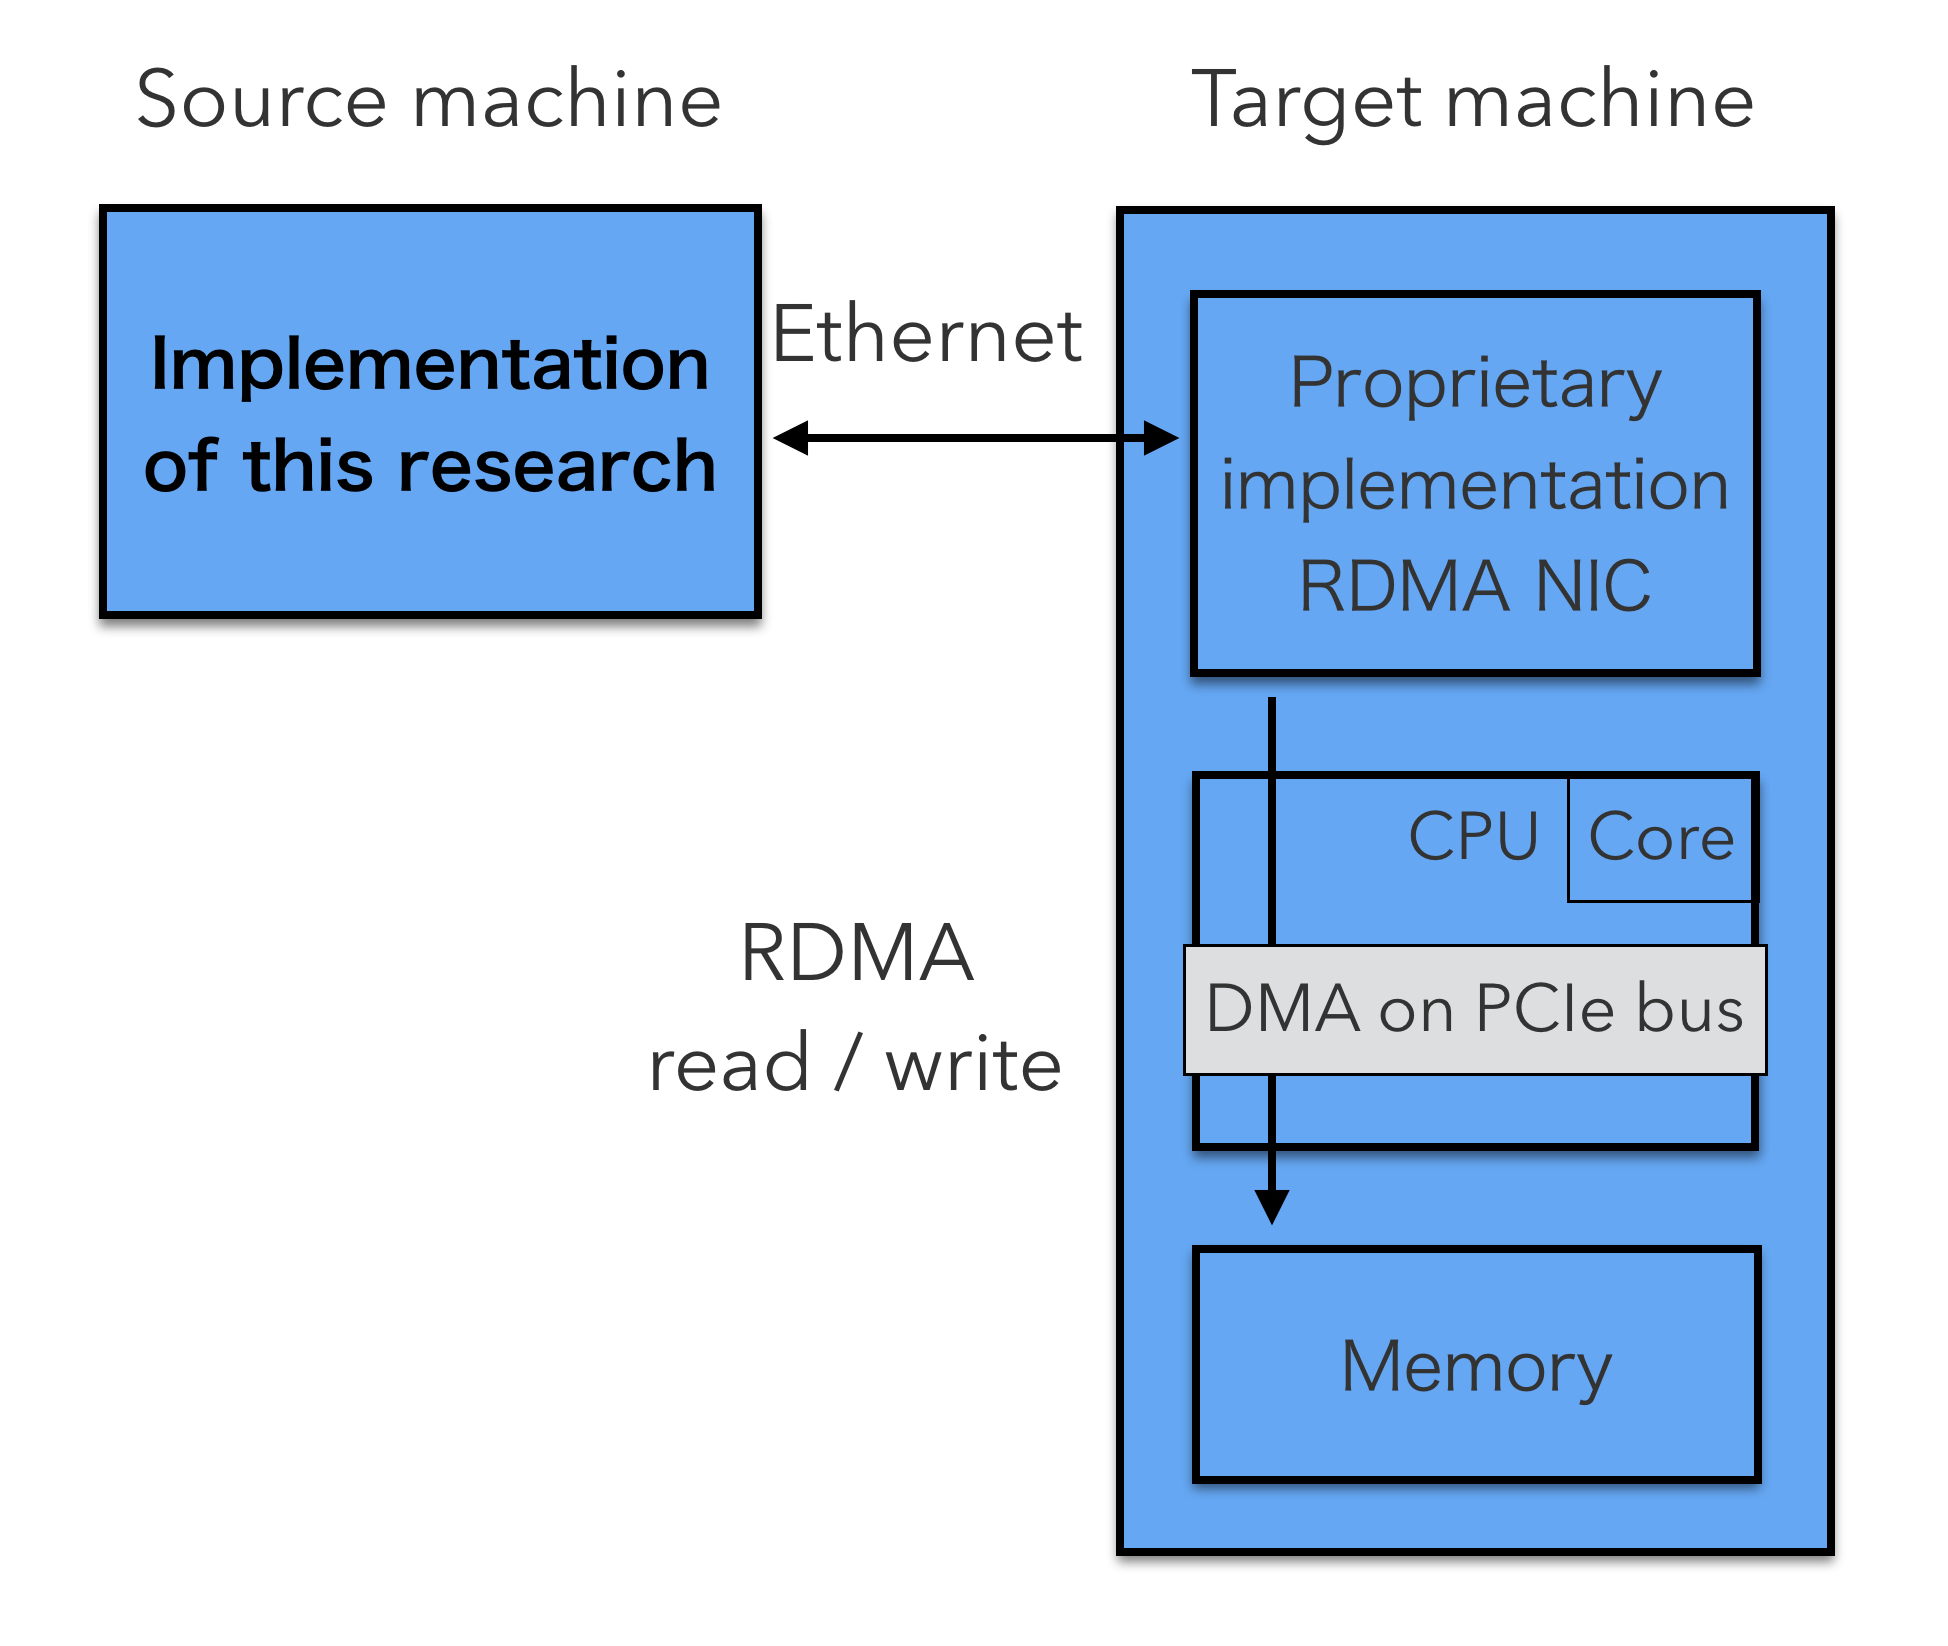
\includegraphics[bb=0 0 1000 530,width=15cm]{img/zentai.png}
    \end{center}
\end{figure}

\section{物理アドレスを指定したメモリの値の取得}

ここにどのように叩くと値が返ってくるかを書く

\section{実装の全体}

ダンプしてくるということを書く.物理アドレスのマッピングに関しても

次の工程として,収集したカーネルコンフィグを元に手元のコンピュータでLinuxカーネルのソースコードに対してプリプロセスの処理を行い,task_struct型を確定する.
さらに,ソースコード上にある__phys_addrの実体を収集する.

最後に,この工程で得られた情報をもとに,libtlpで提唱されている手法を用いて,プロセスの一覧を正しく取得できることを確認する.

\section{工程1}

第一の工程として,RDMA NICを用いて,監視対象ホストのメモリを全探索し,メモリに落ちているSystem.mapのうち,init_taskが配置されている仮想アドレス空間に関する情報と,
Linuxカーネルにおける__phys_addr関数,task_struct型を決定するためのカーネルコンフィグに関する情報を収集することは\ref{chap:related_works}章で述べた.

(本セクションでは,その実装を詳しく書く.ダンプしまくるやつの説明をここに書く)

\section{工程2}

収集したカーネルコンフィグを元に手元のコンピュータでLinuxカーネルのソースコードに対してプリプロセスの処理を行い,task_struct型を確定する.
さらに,ソースコード上にある__phys_addrの実体を収集する部分に関する実装をより詳しく書く.

\section{工程3}

最後に,集められたデータをもとに,process-listを改造したものに関する説明をここに書く
